% ========================================
%	Header einbinden
% ========================================

\documentclass[bibtotoc,titlepage]{scrartcl}

% Deutsche Spracheinstellungen
\usepackage[ngerman,german]{babel, varioref}
\usepackage[T1]{fontenc}
\usepackage[utf8]{inputenc}

%\usepackage{marvosym}

\usepackage{amsfonts}
\usepackage{amssymb}
\usepackage{amsmath}
\usepackage{amscd}
\usepackage{amstext}

\usepackage{longtable}

%\usepackage{bibgerm}

\usepackage{footnpag}

\usepackage{ifthen}                 %%% package for conditionals in TeX
\usepackage[amssymb]{SIunits}
%Für textumflossene Bilder und Tablellen
%\usepackage{floatflt} - veraltet

%Für Testzwecke aktivieren, zeigt labels und refs im Text an.
%\usepackage{showkeys}

% Abstand zwischen zwei Absätzen nach DIN (1,5 Zeilen)
% \setlength{\parskip}{1.5ex plus0.5ex minus0.5ex}

% Einrückung am Anfang eines neuen Absatzes nach DIN (keine)
%\setlength{\parindent}{0pt}

% Ränder definieren
% \setlength{\oddsidemargin}{0.3cm}
% \setlength{\textwidth}{15.6cm}

% bessere Bildunterschriften
%\usepackage[center]{caption2}


% Problemlösungen beim Umgang mit Gleitumgebungen
\usepackage{float}

% Nummeriert bis zur Strukturstufe 3 (also <section>, <subsection> und <subsubsection>)
%\setcounter{secnumdepth}{3}

% Führt das Inhaltsverzeichnis bis zur Strukturstufe 3
%\setcounter{tocdepth}{3}
\usepackage[version=3]{mhchem}
	\mhchemoptions{minus-sidebearing-left=0.06em, minus-sidebearing-right=0.11em}
\usepackage{exscale}

\newenvironment{dsm} {\begin{displaymath}} {\end{displaymath}}
\newenvironment{vars} {\begin{center}\scriptsize} {\normalsize \end{center}}


\newcommand {\en} {\varepsilon_0}               % Epsilon-Null aus der Elektrodynamik
\newcommand {\lap} {\; \mathbf{\Delta}}         % Laplace-Operator
\newcommand {\R} { \mathbb{R} }                 % Menge der reellen Zahlen
\newcommand {\e} { \ \mathbf{e} }               % Eulersche Zahl
\renewcommand {\i} { \mathbf{i} }               % komplexe Zahl i
\newcommand {\N} { \mathbb{N} }                 % Menge der nat. Zahlen
\newcommand {\C} { \mathbb{C} }                 % Menge der kompl. Zahlen
\newcommand {\Z} { \mathbb{Z} }                 % Menge der kompl. Zahlen
\newcommand {\limi}[1]{\lim_{#1 \rightarrow \infty}} % Limes unendlich
\newcommand {\sumi}[1]{\sum_{#1=0}^\infty}
\newcommand {\rot} {\; \mathrm{rot} \,}         % Rotation
\newcommand {\grad} {\; \mathrm{grad} \,}       % Gradient
\newcommand {\dive} {\; \mathrm{div} \,}        % Divergenz
\newcommand {\dx} {\; \mathrm{d} }              % Differential d
\newcommand {\cotanh} {\; \mathrm{cotanh} \,}   %Cotangenshyperbolicus
\newcommand {\asinh} {\; \mathrm{areasinh} \,}  %Area-Sinus-Hyp.
\newcommand {\acosh} {\; \mathrm{areacosh} \,}  %Area-Cosinus-H.
\newcommand {\atanh} {\; \mathrm{areatanh} \,}  %Area Tangens-H.
\newcommand {\acoth} {\; \mathrm{areacoth} \,}  % Area-cotangens
\newcommand {\Sp} {\; \mathrm{Sp} \,}
\newcommand {\mbe} {\stackrel{\text{!}}{=}}     %Must Be Equal
\newcommand{\qed} { \hfill $\square$\\}
\renewcommand{\i} {\imath}
\def\captionsngerman{\def\figurename{\textbf{Abb.}}}

%%%%%%%%%%%%%%%%%%%%%%%%%%%%%%%%%%%%%%%%%%%%%%%%%%%%%%%%%%%%%%%%%%%%%%%%%%%%
% SWITCH FOR PDFLATEX or LATEX
%%%%%%%%%%%%%%%%%%%%%%%%%%%%%%%%%%%%%%%%%%%%%%%%%%%%%%%%%%%%%%%%%%%%%%%%%%%%
%%%
\ifx\pdfoutput\undefined %%%%%%%%%%%%%%%%%%%%%%%%%%%%%%%%%%%%%%%%% LATEX %%%
%%%
\usepackage[dvips]{graphicx}       %%% graphics for dvips
\DeclareGraphicsExtensions{.eps,.ps}   %%% standard extension for included graphics
\usepackage[ps2pdf]{thumbpdf}      %%% thumbnails for ps2pdf
\usepackage[ps2pdf,                %%% hyper-references for ps2pdf
bookmarks=true,%                   %%% generate bookmarks ...
bookmarksnumbered=true,%           %%% ... with numbers
hypertexnames=false,%              %%% needed for correct links to figures !!!
breaklinks=true,%                  %%% breaks lines, but links are very small
linkbordercolor={0 0 1},%          %%% blue frames around links
pdfborder={0 0 112.0}]{hyperref}%  %%% border-width of frames
%                                      will be multiplied with 0.009 by ps2pdf
%
\hypersetup{ pdfauthor   = {Hannes Franke; Julius Tilly},
pdftitle    = {V301 Innenwiderstand und Leistungsanpassung}, pdfsubject  = {Protokoll FP}, pdfkeywords = {V301, Innenwiderstand, Leistungsanpassung},
pdfcreator  = {LaTeX with hyperref package}, pdfproducer = {dvips
+ ps2pdf} }
%%%
\else %%%%%%%%%%%%%%%%%%%%%%%%%%%%%%%%%%%%%%%%%%%%%%%%%%%%%%%%%% PDFLATEX %%%
%%%
\usepackage[pdftex]{graphicx}      %%% graphics for pdfLaTeX
\DeclareGraphicsExtensions{.pdf}   %%% standard extension for included graphics
\usepackage[pdftex]{thumbpdf}      %%% thumbnails for pdflatex
\usepackage[pdftex,                %%% hyper-references for pdflatex
bookmarks=true,%                   %%% generate bookmarks ...
bookmarksnumbered=true,%           %%% ... with numbers
hypertexnames=false,%              %%% needed for correct links to figures !!!
breaklinks=true,%                  %%% break links if exceeding a single line
linkbordercolor={0 0 1},
linktocpage]{hyperref} %%% blue frames around links
%                                  %%% pdfborder={0 0 1} is the default
\hypersetup{
pdftitle    = {V301 Innenwiderstand und Leistungsanpassung}, 
pdfsubject  = {Protokoll AP}, 
pdfkeywords = {V301, Innenwiderstand, Leistungsanpassung},
pdfsubject  = {Protokoll AP},
pdfkeywords = {V301, Innenwiderstand, Leistungsanpassung}}
%                                  %%% pdfcreator, pdfproducer,
%                                      and CreationDate are automatically set
%                                      by pdflatex !!!
\pdfadjustspacing=1                %%% force LaTeX-like character spacing
\usepackage{epstopdf}
%
\fi %%%%%%%%%%%%%%%%%%%%%%%%%%%%%%%%%%%%%%%%%%%%%%%%%%% END OF CONDITION %%%
%%%%%%%%%%%%%%%%%%%%%%%%%%%%%%%%%%%%%%%%%%%%%%%%%%%%%%%%%%%%%%%%%%%%%%%%%%%%
% seitliche Tabellen und Abbildungen
%\usepackage{rotating}
\usepackage{ae}
\usepackage{
  array,
  booktabs,
  dcolumn
}
\makeatletter 
  \renewenvironment{figure}[1][] {% 
    \ifthenelse{\equal{#1}{}}{% 
      \@float{figure} 
    }{% 
      \@float{figure}[#1]% 
    }% 
    \centering 
  }{% 
    \end@float 
  } 
  \makeatother 


  \makeatletter 
  \renewenvironment{table}[1][] {% 
    \ifthenelse{\equal{#1}{}}{% 
      \@float{table} 
    }{% 
      \@float{table}[#1]% 
    }% 
    \centering 
  }{% 
    \end@float 
  } 
  \makeatother 
%\usepackage{listings}
%\lstloadlanguages{[Visual]Basic}
%\allowdisplaybreaks[1]
%\usepackage{hycap}
%\usepackage{fancyunits}


% ========================================
%	Angaben für das Titelblatt
% ========================================

\title{Versuch 701 - Reichweite von $\alpha$-Strahlung\\				% Titel des Versuchs 
\large TU Dortmund, Fakultät Physik\\ 
\normalsize Anfänger-Praktikum}

\author{Jan Adam\\			% Name Praktikumspartner A
{\small \href{jan.adam@tu-dortmund.de}{jan.adam@tu-dortmund.de}}	% Erzeugt interaktiven einen Link
\and						% um einen weiteren Author hinzuzfügen
Dimitrios Skodras\\					% Name Praktikumspartner B
{\small \href{dimitrios.skodras@tu-dortmund.de}{dimitrios.skodras@tu-dortmund.de}}		% Erzeugt interaktiven einen Link
}
\date{18. Juni 2013}				% Das Datum der Versuchsdurchführung

% ========================================
%	Das Dokument beginnt
% ========================================

\begin{document}

% ========================================
%	Titelblatt erzeugen
% ========================================

\maketitle					% Jetzt wird die Titelseite erzeugt
\thispagestyle{empty} 				% Weder Kopfzeile noch Fußzeile

% ========================================
%	Der Vorspann
% ========================================

%\newpage					% Wenn Verzeichnisse auf einer neuen Seite beginnen sollen
%\pagestyle{empty}				% Weder Kopf- noch Fußzeile für Verzeichnisse

\tableofcontents

%\newpage					% eine neue Seite
%\thispagestyle{empty}				% Weder Kopf- noch Fußzeile für Verzeichnisse
%\listoffigures					% Abbildungsverzeichnis

%\newpage					% eine neue Seite
%\thispagestyle{empty}				% Weder Kopf- noch Fußzeile für Verzeichnisse
%\listoftables					% Tabellenverzeichnis
\newpage					% eine neue Seite


% ========================================
%	Kapitel
% ========================================

\section{Einleitung}				% Bei Bedarf
\setcounter{page}{1}
Bei radioaktiven Zerfällen entstehen je nach Nuklid verschiedene Strahlungen, wie auch die sogenannte $\alpha$-Strahlung. Im Verlauf
des Experiments soll ihre Reichweite in Luft ermittelt werden.
\section{Theorie}
\subsection{Bethe-Bloch-Gleichung}
Ein $\alpha$-Teilchen ist ein zweifach positiv geladener $^4_2$He-Kern, der beim gleichnamigen $\alpha$-Zerfall von einem radioaktiven
Atom emittiert wird. Durch die Coulomb-Abstoßung des zerfallenen Kerns erhält der Heliumkern kinetische Energie $E_\alpha$. Die zu bestimmende
Reichweite wird beim Durchschreiten von Materie von verschiedenen Effekten beeinflusst. Zum einen treten elastische Stöße zwischen den
$\alpha$-Teilchen und der Materie auf, wenn es auch einen gerinen Einfluss hat. Weiterhin kann die Energie neben Ionisation auch durch
Anregung und Dissoziation von Molekülen abgegeben werden. Der Verlust an Energie auf einer Wegstrecke $x$ hängt von der anfänglichen
Energie, sowie von der Dichte des Mediums $\rho$ ab. Für hinreichend große Energien beschreibt die Bethe-Bloch-Gleichung diesen Verlust
durch
\begin{align}
 -\frac{\dx E_\alpha}{\dx x} = \frac{z^2 \, e^4}{4 \pi \epsilon_0 \,m_e} \frac{nZ}{v^2}\, \ln \left(\frac{2 m_e v^2}{I}\right),
 \label{eq_bethebloch}
\end{align}
mit Ladung $z$ und Geschwindigkeit $v$ der $\alpha$-Strahlung. $Z$ ist die Ordnungszahl, $n$ die Teilchendichte und $I$ die Ionisationsenergie
des Targetgases. Gleichung \eqref{eq_bethebloch} verliert bei sehr kleinen Energien ihre Gültigkeit aufgrund von Ladungsaustauschprozessen.
Die gesuchte Reichweite $R$ ist die Distanz von Quelle bis zur völligen Abbremsung und wird ermittelt durch
\begin{align}
 R = \int\limits_0^{E_\alpha} -\frac{\dx E_\alpha}{\dx E_\alpha / \dx x}
 \label{eq_reichweite_integral}
\end{align}

\subsection{Empirische, mittlere Reichweite}
Wegen dem Gültigkeitsbereich von \eqref{eq_bethebloch}, welcher nicht in der Auswertung erreicht wird, nimmt man eine empirisch gewonnene
Gleichung, um die mittlere Reichweite $R_m$ zu bestimmen. Das ist jene Reichweite, die die Hälfte der der $\alpha$-Teilchen erreicht.
\begin{align}
 R_m = 3,1\cdot E^{3/2}_\alpha  \hspace{1cm} R_m \, \text{in mm und}\, E_\alpha\, \text{in MeV}
 \label{eq_reichweite_empirisch}
\end{align}
Die Reichweite ist bei konstanter Temperatur und konstantem Volumen proportional zum Druck $p$. Für den Abstand $x_0$ zwischen Quelle und Detektor
gilt für die effektive Weglänge $x$ die Beziehung
\begin{align}
 x = x_0 \frac{p}{p_0} \hspace{1cm} p_0 = 1013\, \text{mbar},
 \label{eq_reichweite_auswertung}
\end{align}
wobei $p_0$ der Normaldruck ist. 

\subsection{Wahrscheinlichkeitsverteilungen}
Die Wahrscheinlichkeit für einen Kern, ein $\alpha$-Teilchen zu emittieren folgt zwei möglichen Verteilungen. Die Gauss-Verteilung gibt
die Wahrscheinlichkeit $P(x)$ an, für eine stetige Messgröße $x$. Die Verteilung ergibt sich, wenn $x$ einer zufälligen Verteilung um den Mittelwert
$\mu$ folgt. Berechnet wird die Wahrscheinlichkeit durch
\begin{align}
 P(x) = \frac{1}{\sqrt{2\pi}\sigma} \e^{\frac12\left(\frac{x-\mu}{\sigma} \right)^2},
 \label{eq_gauss}
\end{align}
mit $\sigma$ als Varianz. Die Poisson-Verteilung ist eine Verteilung für Ereignisse, deren Eintrittswahrscheinlichkeit in einem gegebenen
Intervall sehr klein ist. Die Wahrscheinlichkeit für das $k$-malige Auftreten eines Ereignisses ist gegeben durch
\begin{align}
 P(k) = \frac{\mu^k}{k!}\e^{-\mu}.
 \label{eq_poisson}
\end{align}
Der Parameter $\mu$ ist hierbei gleichzeitig Mittelwert und Varianz.

\section{Durchführung}
\subsection{Reichweite von $\alpha$-Strahlung}
Für zwei Abstände werden Anzahl und Energie, der im evakuierten Glaszylinder pro Sekunde auf die Sonde auftreffenden $\alpha$-Teilchen gemessen. Die Messzeit beträgt 120 Sekunden. Nach jeder Messung wird der Druck im Gefäß erhöht. Gemessen wird im Bereich zwischen (0 - 1000)mbar.\\

\subsection{Statistik des radioaktiven Zerfalls}
Es soll die Verteilung des radioaktiven Zerfalls untersucht werden. Hierzu wird 150 mal über 10 Sekunden die Anzahl der auftreffenden Teilchen gemessen und die daraus ermittelten Zerfallsraten in ein Histogramm eingezeichnet.\\
Das so entstandene Histogramm wird anschließend mit einer Gauß- und einer Poissonverteilung verglichen.
\section{Auswertung}
\subsection{Fehlerrechnung}
Um die Fehler der ermittelten Größen zu bestimmen, werden der Mittelwert
\begin{formel}[H]
\begin{equation}
 \bar{x} = \frac1N \sum_{i=1}^{N} x_i,
 \label{eq_mittel}
\end{equation}
\caption*{\small{$\bar{x}$ = Mittelwert, N = Anzahl der Messungen}}
\end{formel}
die Gaußsche Fehlerfortpflanzung
\begin{formel}[H]
\begin{equation}
\Delta G = \sqrt{\sum_{i=1}^{N}\left( \frac{\partial G}{\partial x_i}\cdot \Delta x_i\right)^2},
\label{gauss}
\end{equation}
\caption*{$x_i$ = Variable, $\Delta x_i$ = Fehler der Variable}
\end{formel}
und die Standardabweichung des Mittelwerts benötigt.
\begin{equation}
 \bar s = \sqrt{\frac{1}{N(N-1)} \sum_{i}^{N} (x_i - \bar{x})^2}
 \label{eq_standard}
\end{equation}
\newpage
\subsection{Aufgenommene Daten}
In folgenden Tabellen sind die, für den ersten Teil der Durchführung ermittelten Werte eingetragen.
\begin{table}[H]
\renewcommand{\arraystretch}{.95}
\begin{tabular}{|c|c|c|c|} 
Druck [mbar]	&Channel$_{max}$	&$N$	&$\Delta N$\\ \hline
0		&1470	&68552	&571.27\\ \hline
100		&1355	&68560	&571.33\\ \hline
200		&1364	&68018	&566.82\\ \hline
300		&1227	&67923	&566.03\\ \hline
400		&1223	&67088	&559.07\\ \hline
450		&1120	&65628	&546.90\\ \hline
500		&1023	&65997	&549.98\\ \hline
550		&996	&64970	&541.42\\ \hline
600		&1023	&64257	&535.48\\ \hline
650		&824	&64252	&535.43\\ \hline
700		&756	&57766	&481.38\\ \hline
750		&684	&48051	&400.43\\ \hline
800		&600	&30901	&257.51\\ \hline
850		&582	&9003	&75.03\\ \hline
900		&584	&1210	&10.08\\ \hline
950		&608	&125	&1.04\\ \hline
1000	&841	&3		&0.03\\ \hline
\end{tabular}
\renewcommand{\arraystretch}{1}
\caption{Gemessene Werte im Abstand von 2,9cm über 120s}
\end{table}

\begin{table}[H]
\renewcommand{\arraystretch}{.95}
\begin{tabular}{|c|c|c|c|} 
Druck [mbar]	&Channel$_{max}$	&$N$	&$\Delta N$\\ \hline
0	&1318	&59249	&493.74 \\ \hline
100	&1336	&58709	&489.24\\ \hline
200	&1295	&58689	&489.08\\ \hline
300	&1163	&57756	&481.30\\ \hline
400	&1023	&57005	&475.04\\ \hline
450	&1023	&56446	&470.38\\ \hline
500	&1023	&55894	&465.78\\ \hline
550	&896	&54468	&453.90\\ \hline
600	&828	&52393	&436.61\\ \hline
650	&802	&47745	&397.88\\ \hline
700	&660	&37753	&314.61\\ \hline
750	&583	&18326	&152.72\\ \hline
800	&583	&4704	&39.20\\ \hline
850	&621	&152	&1.27\\ \hline
900	&692	&4		&0.03\\ \hline
\end{tabular} 
\renewcommand{\arraystretch}{1}
\caption{Gemessene Werte im Abstand von 3,1cm über 120s}
\end{table}

\subsection{Energie -- Druck}
Entsprechend der Versuchsanleitung wird nun angenommen, dass der für den Druck p=0mbar gemessene Channel einer Energie von 4MeV entspricht und dass eine lineare Abhängigkeit vorliegt. Die Steigung $\Delta E$ beträgt somit:
\begin{align*}
\Delta E_{2,9}=\frac{4}{1470}~[\text{MeV}] = 2,72\cdot10^{-3}[\text{MeV}]\\
\Delta E_{3,1}=\frac{4}{1318}~[\text{MeV}] = 3,03\cdot10^{-3}[\text{MeV}]
\end{align*}

In Abhängigkeit des Druckes ergeben sich damit die Energien wie folgt:\\

\begin{minipage}[t]{0.3\textwidth}
\begin{tabular}{|c|c|c|} 
Druck [mbar]	&Channel$_{max}$	& E [meV]\\ \hline
0		&1470			&4\\ \hline
100		&1355			&3.69\\ \hline
200		&1364			&3.71\\ \hline
300		&1227			&3.34\\ \hline
400		&1223			&3.33\\ \hline
450		&1120			&3.05\\ \hline
500		&1023			&2.78\\ \hline
550		&996			&2.71\\ \hline
600		&1023			&2.78\\ \hline
650		&824			&2.24\\ \hline
700		&756			&2.06\\ \hline
750		&684			&1.86\\ \hline
800		&600			&1.63\\ \hline
850		&582			&1.58\\ \hline
900		&584			&1.59\\ \hline
950		&608			&1.65\\ \hline
1000	&841			&2.29\\ \hline
\end{tabular}
\captionof{table}{\mbox{Energien in 2,9cm}}
\end{minipage}
\hspace{3cm}
\begin{minipage}[t]{0.3\textwidth}
\begin{tabular}{|c|c|c|}
Druck [mbar]	&Channel$_{max}$	& E [meV]\\ \hline
0	&1318			&4\\ \hline
100	&1336			&4.05\\ \hline
200	&1295			&3.93\\ \hline
300	&1163			&3.53\\ \hline
400	&1023			&3.10\\ \hline
450	&1023			&3.10\\ \hline
500	&1023			&3.10\\ \hline
550	&896			&2.72\\ \hline
600	&828			&2.51\\ \hline
650	&802			&2.43\\ \hline
700	&660			&2.00\\ \hline
750	&583			&1.77\\ \hline
800	&583			&1.77\\ \hline
850	&621			&1.88\\ \hline
900	&692			&2.10\\ \hline
\end{tabular}
\captionof{table}{\mbox{Energien in 3,1cm}}
\end{minipage}

\subsection{Zählrate -- effektive Länge}
Die effektive Länge errechnet sich nach Gleichung \eqref{eq_reichweite_auswertung}. Für die hier verwendeten Drücke und Abstände erhält man damit:
\begin{table}[H]
\begin{tabular}{|c|c|c|}
Druck [mbar]	& $x_1$ [cm]	& $x_2$ [cm]\\ \hline
0					&0.00	&0.00\\ \hline
100					&0.29	&0.31\\ \hline
200					&0.57	&0.61\\ \hline
300					&0.86	&0.92\\ \hline
400					&1.15	&1.22\\ \hline
450					&1.29	&1.38\\ \hline
500					&1.43	&1.53\\ \hline
550					&1.57	&1.68\\ \hline
600					&1.72	&1.84\\ \hline
650					&1.86	&1.99\\ \hline
700					&2.00	&2.14\\ \hline
750					&2.15	&2.30\\ \hline
800					&2.29	&2.45\\ \hline
850					&2.43	&2.60\\ \hline
900					&2.58	&2.75\\ \hline
950					&2.72	&2.91\\ \hline
1000				&2.86	&3.06\\ \hline 
\end{tabular} 
\end{table}

Grafisch aufgetragen ergeben sich folgende Kurven:
\begin{figure}[H]
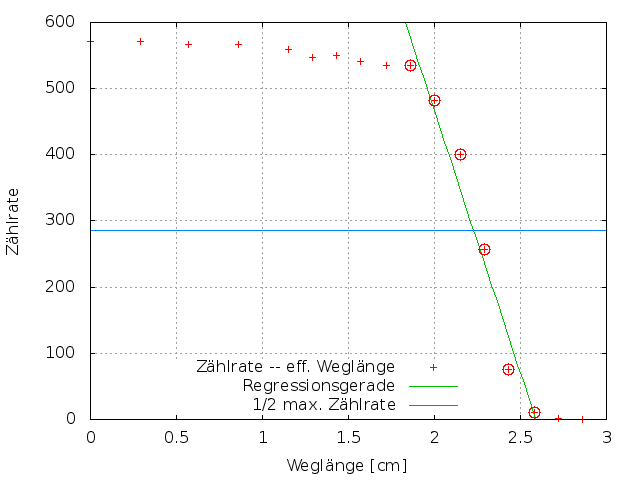
\includegraphics[width=0.8\textwidth]{pics/zaehlrate_weglaenge.png}
\caption{Zählrate gegen die effektive Weglänge aufgetragen im Abstand 2,9cm; die eingekreisten Werte wurden für die lineare Regression verwendet}
\label{pic_zw1}
\end{figure}

\begin{figure}[H]
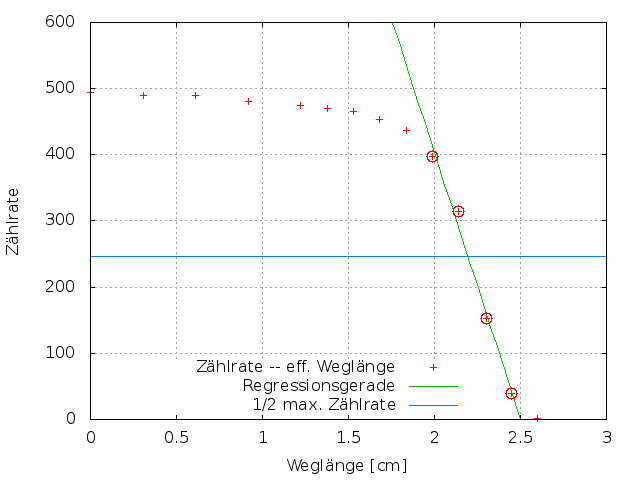
\includegraphics[width=0.8\textwidth]{pics/zaehlrate_weglaenge2.png}
\caption{Zählrate gegen die effektive Weglänge aufgetragen im Abstand 3,1cm; die eingekreisten Werte wurden für die lineare Regression verwendet}
\label{pic_zw2}
\end{figure}

Es soll nun aus den Graphen die mittlere Reichweite der Alphateilchen und damit ihre mittlere Energie bestimmt werden. Hierzu wird eine Regressionsgerade zum linear abfallenden Teil des Graphens gezeichnet und ihr Schnittpunkt mit der halben maximalen Zählrate bestimmt.

Für die hier bestimmten Graphen werden die Regressionsgeraden vom Typ
\begin{align*}
f(x)&=mx+b\\
\end{align*}
bestimmt: 
\subsubsection{Abbildung \ref{pic_zw1}}
\begin{align*}
m&=-792,14 \pm 73,4\\
b&= 2050,54 \pm 163.8
\end{align*}
Die halbe maximale Zählrate beträgt:
\begin{align*}
 \frac{1}{2}\Delta N_{max} = \frac{571.27}{2} = 285,64
\end{align*}
Stellt man die Gleichung um und setzt die halbe maximale Zählrate ein, so erhalt man als mittlere effektive Weglänge:
\begin{align*}
x_{eff1}=\frac{2050,54-285,64}{792,14} = 2,23\pm0,29
\end{align*}
Der Fehler $\Delta x_1$ errechnet sich aus der Gaußschen Fehlerfortpflanzung
\begin{align*}
\Delta x_1&=\sqrt{\left(\frac{1}{792,14}\Delta b\right)^2+\left(\frac{285,64-2050,54}{792,14^2}\right)^2}\\ 
&= 0,29
\end{align*}
Dies entspricht einer Energie von etwa 1,7MeV.

\subsubsection{Abbildung \ref{pic_zw2}}
\begin{align*}
m&=-804,79 \pm 59,64\\
b&= 2012,73  \pm 132,8
\end{align*}
Die halbe maximale Zählrate beträgt:
\begin{align*}
 \frac{1}{2}\Delta N_{max} = \frac{493.74}{2} = 246,87
\end{align*}
Stellt man die Gleichung um und setzt die halbe maximale Zählrate ein, so erhalt man als mittlere effektive Weglänge:
\begin{align*}
x_{eff1}=\frac{2012,73-246,87}{804,79} = 2,19\pm0,17
\end{align*}
Der Fehler $\Delta x_2$ errechnet sich aus der Gaußschen Fehlerfortpflanzung
\begin{align*}
\Delta x_2&=\sqrt{\left(\frac{1}{804,79}\Delta b\right)^2+\left(\frac{246,87-2012,73}{804,79^2}\right)^2}\\ 
&= 0,17
\end{align*}
Dies entspricht einer Energie von etwa 1,8MeV.
\subsection{Energie -- effektive Länge}
Die Energie aufgetragen in Abhängigkeit von der effektiven Länge ergibt folgenden Graphen:

\begin{figure}[H]
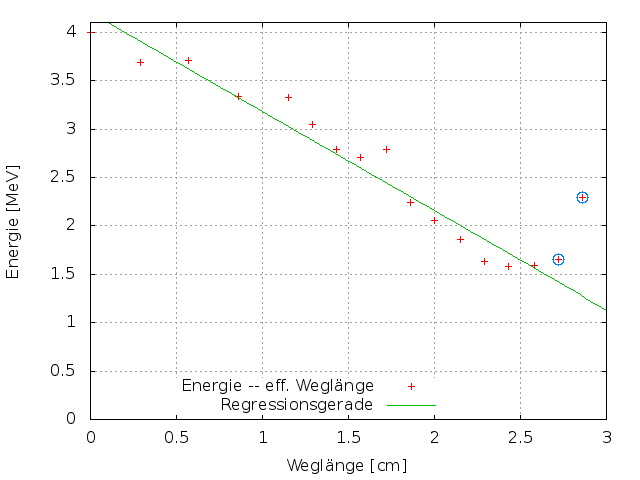
\includegraphics[width=0.8\textwidth]{pics/energie_weglaenge.png}
\caption{Energer gegen die effektive Länge aufgetragen; die eingekreisten Werte wurden nicht für die Regression verwendet}
\end{figure}
Die Steigung der Regressionsgeraden entspricht $-\frac{\Delta E}{\Delta x}$ und wurde mit Gnuplot bestimmt.
\begin{align*}
-\frac{\Delta E}{\Delta x} = 1.03   \pm 0.063
\end{align*}
\subsection{Statistik des radioaktiven Zerfalls}
Um die Statistik des radioaktiven Zerfalls zu überprüfen, wurde 150mal die Zerfallsrate bestimmt und anschließend der Mittelwert, sowie die Standartabweichung berechnet. Die Werte finden sich in Tabelle \ref{tab_zaehlraten}\\
\begin{align*}
\overline{x}&=464,22\\
\sigma&=12,04
\end{align*}

\begin{table}[H]
\begin{tabular}{|c|c|c|c|c|}
\hline 
468,5	&461,1	&473,2	&459,4	&488,6\\ \hline
465,2	&461,6	&471,1	&462,3	&465,2\\ \hline
457,8	&450,3	&449,5	&446,7	&478,5\\ \hline
498,6	&470,4	&448,2	&466,4	&472,0\\ \hline
472,9	&488,2	&470,2	&475,9	&456,3\\ \hline
461,8	&464,9	&474,0	&437,6	&452,3\\ \hline
485,4	&443,4	&463,5	&443,2	&463,2\\ \hline
474,4	&463,4	&473,9	&454,9	&470,1\\ \hline
454,4	&475,8	&488,6	&477,9	&460,2\\ \hline
473,4	&478,3	&448,5	&485,5	&463,5\\ \hline
473,2	&456,9	&467,4	&455,0	&451,8\\ \hline
437,1	&494,9	&459,2	&461,4	&441,2\\ \hline
471,7	&447,8	&448,2	&451,0	&460,0\\ \hline
474,3	&459,7	&457,8	&465,0	&463,6\\ \hline
447,5	&477,9	&471,8	&460,9	&461,4\\ \hline
456,3	&469,4	&475,1	&455,0	&459,1\\ \hline
433,0	&454,7	&440,2	&458,8	&460,8\\ \hline
474,2	&458,8	&465,1	&470,5	&459,6\\ \hline
461,3	&435,9	&456,9	&481,3	&464,7\\ \hline
451,9	&454,2	&461,0	&475,4	&465,0\\ \hline
470,8	&473,3	&473,8	&465,6	&480,2\\ \hline
466,7	&447,2	&491,0	&467,7	&469,9\\ \hline
467,8	&466,9	&480,4	&473,3	&471,1\\ \hline
468,3	&465,4	&463,6	&452,5	&469,7\\ \hline
466,7	&477,0	&461,6	&448,2	&458,7\\ \hline
463,1	&464,2	&465,6	&463,0	&453,0\\ \hline
470,9	&469,4	&459,9	&438,8	&454,7\\ \hline
469,1	&465,2	&493,9	&469,1	&462,8\\ \hline
464,5	&476,9	&462,4	&468,6	&453,5\\ \hline
468,0	&458,6	&474,9	&459,3	&461,2\\ \hline 
\end{tabular} 
\caption{für Auswertung benutze 150 Zählraten, Messzeit 10s}
\label{tab_zaehlraten}
\end{table}

Die Werte werden in ein Histogramm eingetragen. Aufgeteilt wird der Bereich in 5 Abschnitte à 13,2 $\approx \sigma$
\begin{table}[H]
\begin{tabular}{c|c|c|}
Bereich	&Anzahl&	Prozent\\ \hline 
433-446	&9	&6,00\\ \hline
447-459	&30	&20,00\\ \hline
460-473	&76	&50,67\\ \hline
474-486	&28	&18,67\\ \hline
487-499	&7	&4,67\\ \hline\hline
Summe	&150	&100  
\end{tabular} 
\end{table}

\begin{figure}[H]
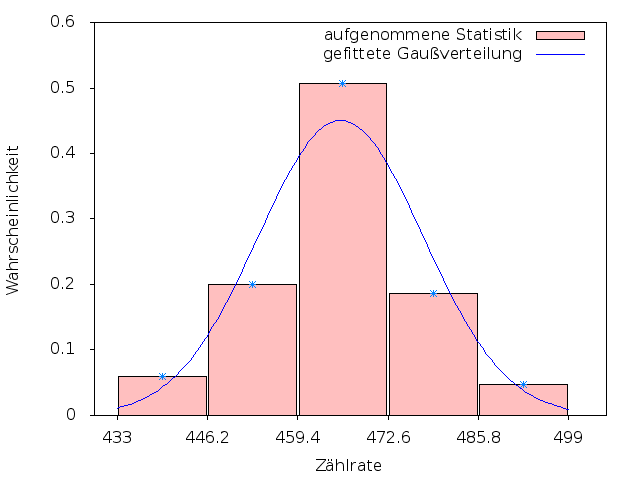
\includegraphics[width=0.75\textwidth]{pics/Gauss.png}
\caption{Histogramm der aufgenommenen Werte, zusammen mit der gefitteten Gaußverteilung}
\end{figure}

\begin{figure}[H]
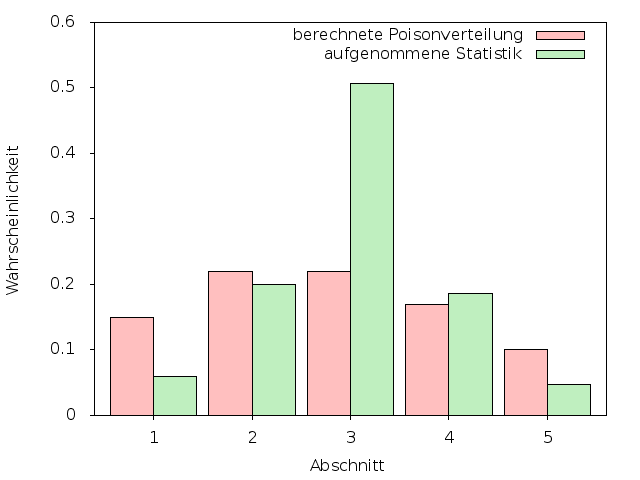
\includegraphics[width=0.75\textwidth]{pics/poisson.png}
\caption{Histogramm der aufgenommenen Werte, zusammen mit der entsprechenden Poissonverteilung}
\end{figure}

\section{Diskussion}
Die experiment bestimmten Reichweiten der Alphastrahlung liegen im Bereich weniger Zentimeter. Dies stimmt mit den theoretischen Behauptungen sehr gut überein.\\

Betrachtet man Abbildungen 4 und 5 kann man weiterhin sagen, dass sowohl die Gaußverteilung, als auch die Poissonverteilung die Statistik des radioaktiven Zerfalls treffend beschreiben. Kleinere Abweichungen der Messwerte vom idealen Graphen sind vorallem darauf zurückzuführen, dass mit n=150 noch lange nicht genug Messwerte aufgenommen worden sind. In diesem Fall würden sich die Messwerte dem Graphen weiter annähern.



% ========================================
%	Literaturverzeichnis
% ========================================

%\bibliographystyle{plainnat}			% Bibliographie-Style auswählen
%\bibliography{BIBDATEI}			% Literaturverzeichnis

% ========================================
%	Das Dokument endent
% ========================================

\end{document}
